\documentclass{article}
%\usepackage[margin=1in]{geometry}
\setlength\topmargin{0pt}
\addtolength\topmargin{-\headheight}
\addtolength\topmargin{-\headsep}
\setlength\oddsidemargin{0pt}
\setlength\textwidth{\paperwidth}
\addtolength\textwidth{-2in}
\setlength\textheight{\paperheight}
\addtolength\textheight{-2in}

\usepackage[english]{babel}
\usepackage[utf8]{inputenc}
\usepackage{fancyhdr}
\usepackage{listings}
\usepackage{graphicx}
\usepackage{xcolor}


\definecolor{codegreen}{rgb}{0,0.6,0}
\definecolor{codegray}{rgb}{0.5,0.5,0.5}
\definecolor{codepurple}{rgb}{0.58,0,0.82}
\definecolor{backcolour}{rgb}{0.95,0.95,0.92}


\usepackage{booktabs}
\usepackage{pgfplotstable}



\lstdefinestyle{mystyle}{
	backgroundcolor=\color{backcolour},
	commentstyle=\color{codegreen},
	keywordstyle=\color{magenta},
	numberstyle=\tiny\color{codegray},
	stringstyle=\color{codepurple},
	basicstyle=\ttfamily\footnotesize,
	breakatwhitespace=false,
	breaklines=true,
	captionpos=b,
	keepspaces=true,
	numbers=left,
	numbersep=5pt,
	showspaces=false,
	showstringspaces=false,
	showtabs=false,
	tabsize=2
}
\lstset{style=mystyle}

\title{Machine Learning Project 3 Neural Networks}
\author{Pedram Safaei, Ian Grant }
\date{December 2nd}

\begin{document}

\maketitle

\section{compute\_Z}
explanation
\begin{lstlisting}[language=Python]
sample code 
\end{lstlisting}


\section{compute\_covariance\_matrix}
explanation
\begin{lstlisting}[language=Python]
sample code 
\end{lstlisting}

\section{find\_pcs}
explanation
\begin{lstlisting}[language=Python]
sample code 
\end{lstlisting}

\section{project\_data}
explanation
\begin{lstlisting}[language=Python]
sample code 
\end{lstlisting}

\section{compress\_images}
explanation
\begin{lstlisting}[language=Python]
sample code 
\end{lstlisting}

\section{load\_data}
explanation
\begin{lstlisting}[language=Python]
sample code 
\end{lstlisting}

\section{Compressed images from DATA/TRAIN}
\subsection{10}
\subsection{100}
\subsection{500}
\subsection{1000}
\subsection{2000}




% 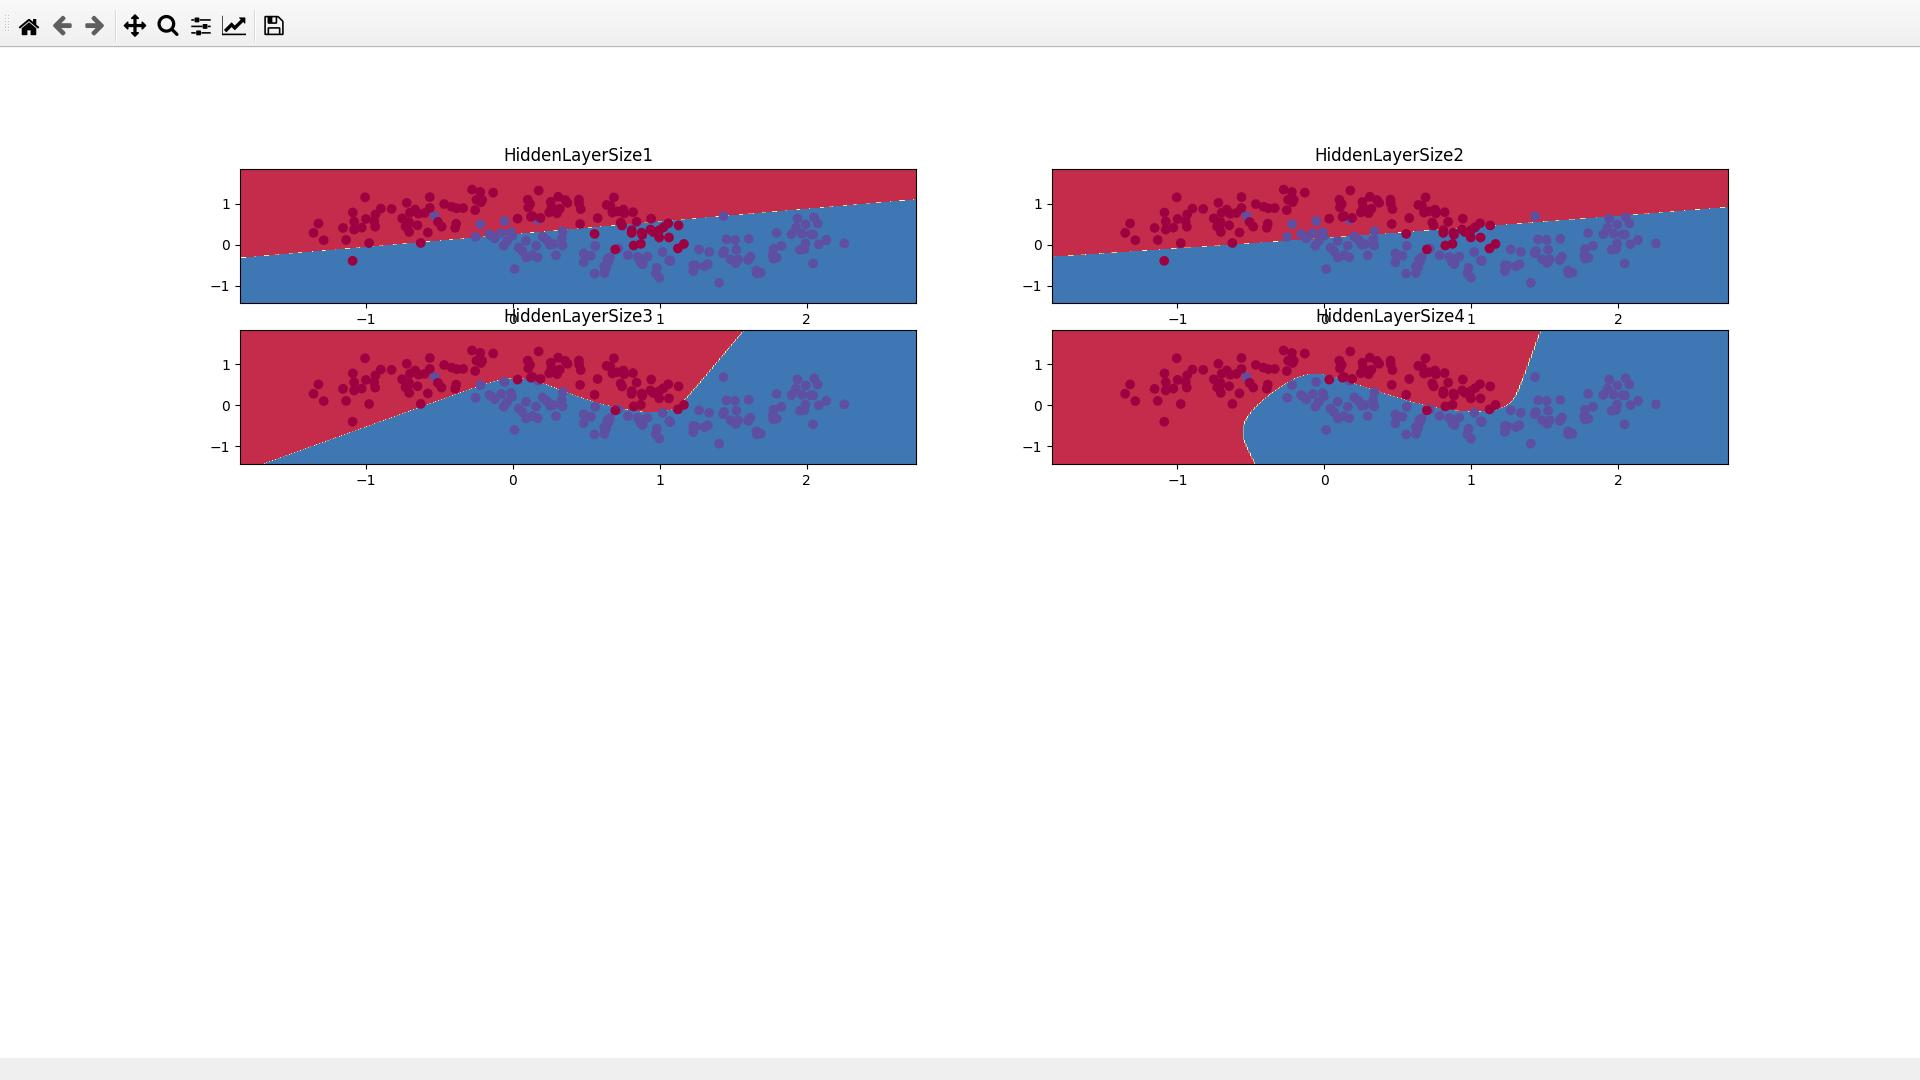
\includegraphics[scale=.25]{plot.jpg}
\end{document}
